\section{Problem 2}

\subsection{Question}
Re-run question 2, but this time with proper TFIDF calculations instead of the hack discussed on slide 7 (p. 32).  Use the same 500 words, but this time replace their frequency count with TFIDF scores as computed in assignment \#3. Document the code, techniques, methods, etc. used to generate these TFIDF values.  Upload the new data file to github.\\
\\
Compare and contrast the resulting dendrogram with the dendrogram from question \#2.\\
\\
Note: ideally you would not reuse the same 500 terms and instead come up with TFIDF scores for all the terms and then choose the top 500 from that list, but I'm trying to limit the amount of work necessary.

\subsection{Answer}
The ascii and jpeg dendrograms were created using the code shown in Listing \ref{listing:clust:main}, which is modeled after the example from class. 

\lstinputlisting[language=Python, caption={creating the dendrograms}, label=listing:clust:main,linerange={286-293},firstnumber=286]{clusters.py}

The {\tt readfile} function shown in Listing \ref{listing:clust:read} was used to read the data that was compiled from Question 1 into memory where it is then processed by the {\tt hcluster} function found in Listing \ref{listing:clust:hclust} to produce the clustered representation of the blogs.

\lstinputlisting[language=Python, caption={creating the dendrograms}, label=listing:clust:read,linerange={3-16},firstnumber=3]{clusters.py}

\lstinputlisting[language=Python, caption={hcluster function}, label=listing:clust:hclust,linerange={48-88},firstnumber=48]{clusters.py}

The {\tt printclust} function from Listing \ref{listing:clust:printclust} prints the ascii dendrogram of the cluster object parameter to sys.stdout, which is redirected to write to a file with the code in Listing \ref{listing:clust:main}.

\lstinputlisting[language=Python, caption={printclust function}, label=listing:clust:printclust,linerange={90-103},firstnumber=90]{clusters.py}

The {\tt drawdendrogram} function from Listing \ref{listing:clust:drawdendro} creates a jpeg image of the cluster, which is shown in Figure \ref{fig:clust}.

\lstinputlisting[language=Python, caption={drawdendrogram function}, label=listing:clust:drawdendro,linerange={122-139},firstnumber=122]{clusters.py}

\begin{figure}[h!]
\centering
\fbox{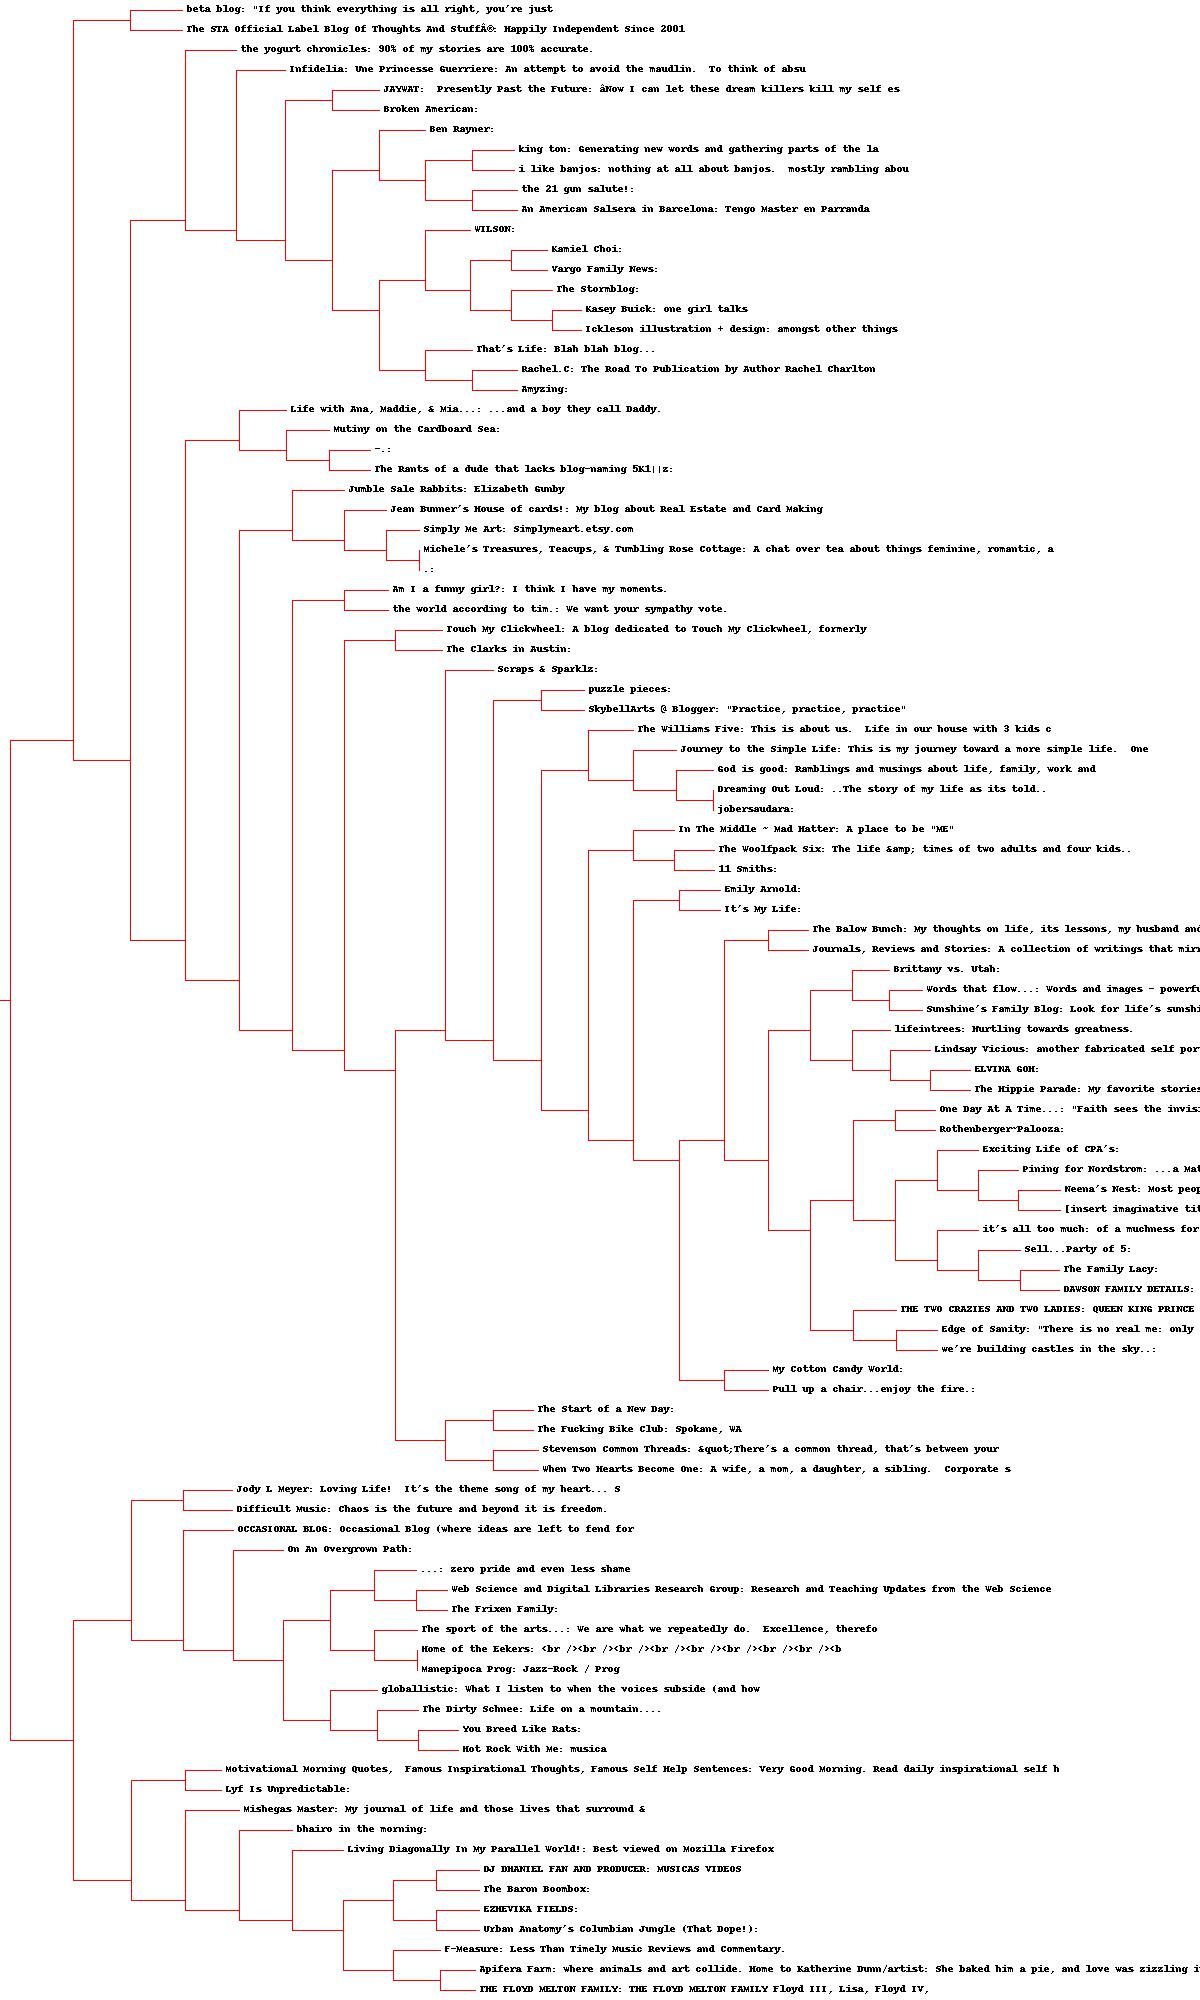
\includegraphics[scale=0.265]{q2/blogclust.jpg}}
\caption{blog dendrogram}
\label{fig:clust}
\end{figure}